\documentclass[letterpaper]{report}
\author{Jonathan Chan\\15354146}
\title{PHYS 319\\One-Octave Recording Piano}

\usepackage{fullpage}
\usepackage{minted}
\usepackage{hyperref}
\usepackage{graphicx}
\usepackage{subcaption}

\begin{document}
	\maketitle
	
	\begin{abstract}
		The goal of this project is to produce a one-octave recording piano. When a button is pressed, it will send a certain input to the microcontroller, which will then interpret the signal as a predetermined pitch and use the PWM to produce a voltage wave with a period corresponding to that pitch. A speaker will then receive this output and play the correct tone. The button is duplicated thirteen times to emulate the thirteen keys in a chromatic octave, from middle C to tenor C. The microcontroller will keep track of which pitches were selected as well as for how long the pitch was sustained by recording overflows of the SMCLK timer the PWM uses, the magnitudes of which are bounded by the memory constraints of the microcontroller. Finally, the recorded song will be played back using the PWM and appropriate delays, triggered by the P1.3 button. A demonstration of these capabilities can be found at \url{https://youtu.be/K61zJs2eH-4}. Some possible improvements and additions to this project could be additional inputs to select the octave, an analogue input whose voltage can be adjusted using a dial and which can be interpreted by the microcontroller's ADC as a volume level, alternative input methods such as a laser and a photodiode to create a rudimentary laser harp, and using both timers of the MSP430 to generate two tones that are added together using an op-amp to create a chord. 
	\end{abstract}

	\chapter{Introduction}
	The goal of this project is to produce a basic functional piano that can record and play a small set of chromatic notes according to a given input. This is based off of the PWM portion of labs 3 and 4, in which we produced a voltage wave with a fixed period that was transduced into a tone with a pitch corresponding to the given frequency. Here, we expand the range of possible tones to a full chromatic octave, which is chosen according to one of the thirteen buttons pressed. The device can also record a song (consisting of a sequence of tones and their lengths) of finite length bounded by the size of the RAM of the microcontroller and play it back.
	
	\chapter{Apparatus}
	The device consists of four major components, physical and programmatic: the keyboard, the speaker, the recorder, and the playback.
		\section{The Keyboard}
			The keyboard consists of thirteen buttons that close a switch when pressed and four dual 4-input OR gate chips that combines them into a four-bit input signal to the microcontroller. The buttons, labelled \texttt{C, Db, D, \dots, G, Ab, \dots, B, C}, need to send the binary inputs \texttt{0001, 0010, \dots, 1100, 1101} respectively (with \texttt{0000} reserved for no tone), so the output of each button is connected to the input of one to three different OR chips, each labelled \texttt{C0, C1, C2, C3}, representing the least to most significant bits. Because the chips have two 4-input gates, the output of one gate is connected to the other, and the output of that gate is connected to the appropriate pin of the microcontroller, from P2.0 to P2.3. 
			
			\begin{figure}[H]
				\centering
				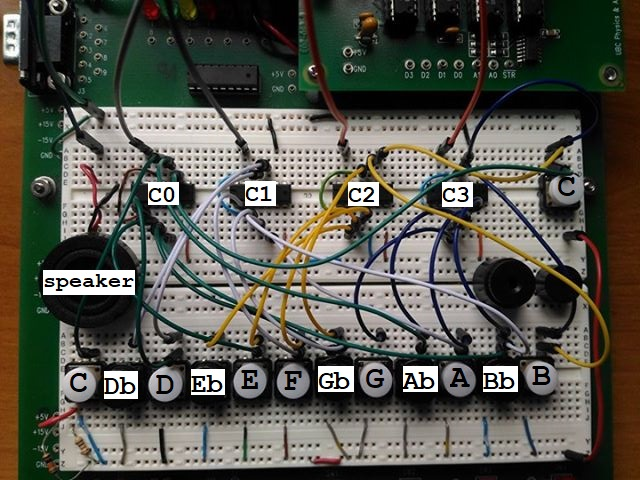
\includegraphics[width=0.73\textwidth]{wiring}
				\caption{Picture of device with labelled buttons and chips.}
			\end{figure}
			
			Below are an example of how the \texttt{Gb} button and the \texttt{C0} chip are wired.
			\begin{figure}[H]
				\centering
				\begin{subfigure}{0.5\textwidth}
					\centering
					
\includegraphics[width=0.4\textwidth]{switch}
					\caption{Circuit diagramme for switch \texttt{Gb}.}
				\end{subfigure}%
				\begin{subfigure}{0.5\textwidth}
					\centering
					
\includegraphics[width=0.8\textwidth]{orgate}
					\caption{Circuit diagramme for OR chip \texttt{C0}.\\ Note that $1 = 2 \vee 3 \vee 4 \vee 5$ and $13 = 12 \vee 11 \vee 10 \vee 9$.}
				\end{subfigure}
				\caption{Circuit diagrammes for a switch and a chip.}
			\end{figure}
			
			% insert circuit diagramme of button and chip
		\section{The Speaker}
			The speaker works the same way as the piezoelectric buzzer from labs 3 and 4: The pitch of the tone emitted is given by the period of the PWM waveform produced. The frequencies of a chromatic scale from middle C to tenor C can be found here \url{https://en.wikipedia.org/wiki/Piano_key_frequencies}; we take the reciprocal of each frequency to find the period, convert it to microseconds, and save the values in an array so that the input corresponds exactly to the index of a tone.
				\begin{minted}{c}
    #define MIDC   3822
    #define DFLAT  3608
    #define D      3405
    #define EFLAT  3214
    #define E      3034
    #define F      2863
    #define GFLAT  2703
    #define G      2551
    #define AFLAT  2408
    #define A      2273
    #define BFLAT  2145
    #define B      2025
    #define TENC   1911
    #define NONE   0
    
    unsigned int scale[16] = {
        NONE,  MIDC, DFLAT, D, EFLAT, E, F, 
        GFLAT, G,    AFLAT, A, BFLAT, B, TENC,
        NONE,  NONE  // should not be used
    };
				\end{minted}
			To play a tone, we mask the input with the bits we need and set the period using the masked input as the index for the scale array. The volume is at its maximum when the duty cycle is exactly half of the period. If the input is 0, we set the period to the maximum (this will become important later on) and set the duty cycle to 0 to silence the playing.
				\begin{minted}{c}				
    void play(unsigned int pitch) {
        if (pitch != 0) {
            CCR0 = scale[pitch];
            CCR1 = scale[pitch] / 2;  // max volume
        } else {
            CCR0 = 0xFFFF;  // cannot count to 0; set to max
            CCR1 = 0;
        }
    }
    
    // in a different function...
    unsigned int pitch = P2IN & 0xF;
    play(pitch);
				\end{minted}
			Finally, we use a while loop to repeatedly check for changes in the input, and play the new tone if it has changed. A delay has been inserted between iterations of the while loop so that input fluctuations that occur while pressing the button don't get picked up.
				\begin{minted}{c}
    unsigned int last_pitch = 0;
    while (recording) {  // recording = true for now
        unsigned int pitch = P2IN & 0xF;
        if (pitch != last_pitch) {
            play(pitch);
            last_pitch = pitch;
        }
        __delay_cycles(1000);
    }
				\end{minted}
		\section{The Recorder} 
			In order to record a song, we not only need to store the sequence of tones that were played, but also the duration for which the tone has been played. There are only thirteen different pitches, so we only need four bits to store it; if we use a bit field in a struct for the pitch, we can use the remaining twelve bits in a word to store the length. For reasons that will be discussed later, the length will be in units of centiseconds, so the maximum length of one note is \texttt{0xFFF} centiseconds, or approximately 41 seconds, which is sufficiently long for most musical applications. 
				\begin{minted}{c}
    // pitch  is index of scale array
    // length is in centiseconds
    // max length of note is 0xFFF = approx. 41 seconds
    typedef struct {
        unsigned int pitch  : 4;
        unsigned int length : 12;
    } Note;
    
    #define MAXNOTES 0xA2   // 162 (not enough RAM to allocate any more to rec)
    Note rec[MAXNOTES];
				\end{minted}
			When compiling, if our \texttt{rec} array is too large, GCC will not compile because it cannot allocate enough memory to it; below is an example error message when \texttt{MAXNOTES} is set to \texttt{0xA3}. The exact value of \texttt{MAXNOTES} was determined to be 162 by trial and error.
				\begin{verbatim}
					/bin/ld: main.elf section `.heap' will not fit in region `RAM'
					/bin/ld: region `RAM' overflowed by 2 bytes
				\end{verbatim}
			The PWM uses the 1 MHz SMCLK clock to count up to the set period, and we can use the same clock to measure elapsed time by setting an interrupt for when the count reaches the maximum. One \texttt{unsigned int} variable is used to store the elapsed time in microseconds; another \texttt{unsigned int} variable is used to store the overflow. Since the maximum value of the variables is \texttt{0xFFFF} = 65536, the overflow variable will store the elapsed time in centiseconds, and for convenience we will increment it by 6 when the microsecond count exceeds 60000. This is also why the length of a note is stored in centiseconds. Because we only expect to store \texttt{0xFFF} centiseconds, there is no need for a second overflow variable.
				\begin{minted}{c}
    // constants used for unit conversions in timer interrupt
    // CSINT should be 256^2 / 10 000 = 65 536 / 10 000 = 6
    // USINT should be 60 000
    #define CSUS   10000    // microseconds (us) in a centisecond (cs)
    #define CSINT  6        // centiseconds storable in int of microseconds
    #define USINT  60000    // CSINT in microseconds
    
    volatile unsigned int us    = 0;
    volatile unsigned int cs    = 0;
    
    #if defined(__TI_COMPILER_VERSION__)
    #pragma vector=TIMER0_A0_VECTOR
    __interrupt void timer0_a0_isr(void)
    #else
        void __attribute__ ((interrupt(TIMER0_A0_VECTOR))) timer0_a0_isr (void)
    #endif
    {
        unsigned int us_left = USINT - us;  // count up to USINT microseconds in us
        if (us_left < TACCR0) {
            cs += CSINT;            // add centiseconds to cs count
            us = TACCR0 - us_left;  // save overflow
        } else {
            us += TACCR0;           // add microseconds to us count
        }
        TACCTL0 &= ~CCIFG;          // set interrupt flag to 0
    }
				\end{minted}
			In the while loop, we then store the new note when it has changed. We also break out of the while loop if we exceed \texttt{MAXNOTES} recorded notes. Note that the recording begins at the second note of the array; we keep the first as \texttt{NONE} of length 0 to have something to compare to in the if statement without it being played in the playback. The \texttt{LED1} helps us see when we are in recording mode.
				\begin{minted}{c}
    volatile bool recording = true;
    volatile unsigned int notes = 1;
    
    void record() {
        TAR = 0;
        P1OUT |= LED1;
        while (recording && notes < MAXNOTES) {
            unsigned int pitch = P2IN & 0xF;
            if (pitch != rec[notes - 1].pitch) {
                rec[notes - 1].length = cs + (us + TAR)/CSUS;
                rec[notes].pitch = pitch;
                play(pitch);
                cs = us = TAR = 0;  // reset all counts
                notes++;
            }
            __delay_cycles(1000);
        }
        P1OUT    &= ~LED1;
        TACCTL0  &= ~CCIE;
        play(0);
    }
				\end{minted}
		\section{The Playback}
			To end the recording and play back the song, we can use the P1.3 button as an interrupt and handle it by cleaning things up and  setting \texttt{recording} to false, then calling the actual playback function. Each press of the interrupt button will trigger a playback (if it is not currently in one), and we can record a different song by pressing the general reset button.
				\begin{minted}{c}
    #if defined(__TI_COMPILER_VERSION__)
    #pragma vector=PORT1_VECTOR
    __interrupt void port1_isr(void)
    #else
        void __attribute__ ((interrupt(PORT1_VECTOR))) port1_isr (void)
    #endif
    {    
        if (recording) {
            rec[notes - 1].length = cs + (us + TAR)/CSUS;
            cs = us = TAR = 0;
            recording = false;
            P1OUT    &= ~LED1;
            TACCTL0  &= ~CCIE;
            play(0);
        }
        playback();
        P1IFG &= ~BUTTON;           // set interrupt flag to 0
    }
				\end{minted}
			The actual playback is straightforward: For each note we have saved, we play the tone, then delay for the appropriate number of centiseconds. 
				\begin{minted}{c}
    void playback() {
        for (unsigned int i = 0; i < notes; i++) {
            play(rec[i].pitch);
            for (unsigned int j = 0; j < rec[i].length; j++) {
                __delay_cycles(CSUS);
            }
        }
    }
				\end{minted}
		Of course, we need to set the special registers appropriately to set inputs, outputs, and clocks. The full code can be found in the appendix of this report.
	\chapter{Procedure and Results}
		The piano can be played by pressing the buttons, and the song played will be recorded. Pressing the P1.3 button will cause the recorded song to be played back. The reset button can be used to begin recording a new song. A video demonstration of the functionality can be found here: \url{https://youtu.be/K61zJs2eH-4}. Both goals of recording and playback have been achieved.
	
	\chapter{Discussion and Conclusion}
		As demonstrated in the video linked to in the previous section, the construction of a one-octave piano with recording abilities was successfully achieved. If we wished to create a more permanent device, we could solder the connections from the switches to the OR gates instead of using jumper wires and breadboards, which would also make it more portable. 
		
		There are, of course, many additional features that could be added to improve its functionality. For instance, many other people who also built pianos included an octave key to change octaves; with three additional switches, it would be possible to cover all octaves of a traditional piano. A volume dial could also be implemented by first amplifying the output signal to the speaker, then adding an analogue input with variable voltage that would be picked up by the microcontroller's ADC and interpreted as some fraction for the duty cycle, which is what determines the volume. The input method could also be altered to emulate a different kinds of instruments; for instance, by replacing each button switch with a laser and a photodiode, we could create a simple laser harp. 
		
		A more advanced feature which would really bring the project closer to a real electric piano would be the ability to play multiple tones simultaneously. Because the MSP430 only has two timers (Timer A and Timer B), we would only be able to generate two simultaneous tones using two PWMs. They would need to be added together using an op-amp as a voltage adder before being sent off to the speaker, which should then play the two-tone chord.
			
	\renewcommand\bibname{References}
	\begin{thebibliography}{9}
		\bibitem{cmos4072}
			\textit{CMOS OR Gates.}
			CD4071B, CD4072B, CD4075B Types.
			Texas Instruments. 
			August 2003.
			\url{http://www.cmos4000.com/media/cmos/ic-cmos-4072.pdf}
		\bibitem{b3f}
			\textit{Tactile Switch.}
			B3F.
			Omron.
			\url{http://omronfs.omron.com/en_US/ecb/products/pdf/en-b3f.pdf}
	\end{thebibliography}
	
	\appendix
	\chapter{Makefile}
		\begin{minted}{Makefile}
    DEVICE  = msp430g2553
    INSTALL_DIR=$(HOME)/ti/msp430_gcc
    
    GCC_DIR =  $(INSTALL_DIR)/bin
    SUPPORT_FILE_DIRECTORY = $(INSTALL_DIR)/include
    
    CC      = $(GCC_DIR)/msp430-elf-gcc
    GDB     = $(GCC_DIR)/msp430-elf-gdb
    
    CFLAGS = -I $(SUPPORT_FILE_DIRECTORY) -mmcu=$(DEVICE) -Os -g
    LFLAGS = -L $(SUPPORT_FILE_DIRECTORY) -T $(DEVICE).ld
    
    all: main.c
        $(CC) $(CFLAGS) $(LFLAGS) $? -o main.elf
        $(CC) $(CFLAGS) $(LFLAGS) $? -S -o main.asm
    
    debug: all
        $(GDB) main.elf
    
    clean:
        rm main.elf main.asm
		\end{minted}
		
	\chapter{main.c}
		\begin{minted}{c}
    #include "msp430.h"
    #include <stdlib.h>
    #include <stdbool.h>
    
    #define MIDC   3822
    #define DFLAT  3608
    #define D      3405
    #define EFLAT  3214
    #define E      3034
    #define F      2863
    #define GFLAT  2703
    #define G      2551
    #define AFLAT  2408
    #define A      2273
    #define BFLAT  2145
    #define B      2025
    #define TENC   1911
    #define NONE   0
    
    #define LED1   BIT0
    #define BUTTON BIT3
    #define OUTPUT BIT6
    
    // constants used for unit conversions in timer interrupt
    // CSINT should be 256^2 / 10 000 = 65 536 / 10 000 = 6
    // USINT should be 60 000
    #define CSUS   10000    // microseconds (us) in a centisecond (cs)
    #define CSINT  6        // centiseconds storable in int of microseconds
    #define USINT  60000    // CSINT in microseconds
    
    #define MAXNOTES 0xA2   // 162 (not enough RAM to allocate any more to rec)
    
    // pitch  is index of scale array
    // length is in centiseconds
    // max length of note is 0xFFF = approx. 41 seconds
    typedef struct {
        unsigned int pitch  : 4;
        unsigned int length : 12;
    } Note;
    
    unsigned int scale[16] = {
        NONE,  MIDC, DFLAT, D, EFLAT, E, F, 
        GFLAT, G,    AFLAT, A, BFLAT, B, TENC,
        NONE,  NONE  // should not be used
    };
    
    Note rec[MAXNOTES];
    volatile bool recording = true;
    volatile unsigned int notes = 1;
    volatile unsigned int us    = 0;
    volatile unsigned int cs    = 0;
    
    void play(unsigned int pitch) {
        if (pitch != 0) {
            CCR0 = scale[pitch];
            CCR1 = scale[pitch] / 2;  // max volume
        } else {
            CCR0 = 0xFFFF;  // cannot count to 0; set to max
            CCR1 = 0;
        }
    }
    
    void playback() {
        for (unsigned int i = 0; i < notes; i++) {
            play(rec[i].pitch);
            for (unsigned int j = 0; j < rec[i].length; j++) {
                __delay_cycles(CSUS);
            }
        }
    }
    
    void save_length(unsigned int position) {
        rec[position].length = cs + (us + TAR)/CSUS;
        cs = us = TAR = 0;  // reset all counts
    }
    
    void end_record() {
        recording = false;
        P1OUT    &= ~LED1;
        TACCTL0  &= ~CCIE;
        play(0);
    }
    
    void record() {
        TAR = 0;
        P1OUT |= LED1;
        while (recording && notes < MAXNOTES) {
            unsigned int pitch = P2IN & 0xF;
            if (pitch != rec[notes - 1].pitch) {
                save_length(notes - 1);
                rec[notes].pitch = pitch;
                play(pitch);
                notes++;
            }
            __delay_cycles(1000);
        }
        end_record();
    }
    
    void main(void) {
        WDTCTL  = WDTPW + WDTHOLD;      // Stop WDT
        
        P2DIR   = 0;                    // P2 all input
        P2REN   = 0xF;                  // P2 inputs resistor enable
        P2OUT   = 0;                    // P2 resistor pulldown
        P1DIR   = OUTPUT | LED1;        // P1.6, P1.0 output (P1.3 input)
        P1SEL  |= OUTPUT;               // P1.6 to TA0.1
        P1REN   = BUTTON;               // button resistor enable
        P1IE    = BUTTON;               // enable button interrupt
        
        CCTL1   = OUTMOD_7;             // CCR1 reset/set
        TACTL   = TASSEL_2 | MC_1;      // SMCLK (1 MHz) count up to CCRO
        TACCTL0 = CCIE;                 // enable clock  interrupt
        
        __enable_interrupt();
        record();
        __bis_SR_register(LPM0_bits);
    }
    
    #if defined(__TI_COMPILER_VERSION__)
    #pragma vector=TIMER0_A0_VECTOR
    __interrupt void timer0_a0_isr(void)
    #else
        void __attribute__ ((interrupt(TIMER0_A0_VECTOR))) timer0_a0_isr (void)
    #endif
    {
        unsigned int us_left = USINT - us;  // count up to USINT microseconds in us
        if (us_left < TACCR0) {
            cs += CSINT;            // add centiseconds to cs count
            us = TACCR0 - us_left;  // save overflow
        } else {
            us += TACCR0;           // add microseconds to us count
        }
        TACCTL0 &= ~CCIFG;          // set interrupt flag to 0
    }
    
    #if defined(__TI_COMPILER_VERSION__)
    #pragma vector=PORT1_VECTOR
    __interrupt void port1_isr(void)
    #else
        void __attribute__ ((interrupt(PORT1_VECTOR))) port1_isr (void)
    #endif
    {    
        if (recording) {
            save_length(notes);
            end_record();
        }
        playback();
        P1IFG &= ~BUTTON;           // set interrupt flag to 0
    }
		\end{minted}
\end{document}